\section{Transformer STN}
\label{sec:Chapter28}

Architektura STN je jedním z možných přístupů jak představit spaciální invarianci do klasických konvolučních neuronových sítí představená v literatuře \cite{stn} roku 2015. Klasické konvoluční neuronové sítě pomocí svých vrstev typu max pooling\footnote{v síti U-Net nacházející se v enkodéru.} tvoří jistou spaciální invarianci proti různým změnám perspektivy, avšak pouze limitovaně. Výrazné transformace vstupního obrazu mívá detrimentální účinek na výslednou robustnost sítě.

Pro adresování této limitace týkající se prostorové invariance vznikla neuronová síť s prostorovým transformerem -- \textbf{STN (ang. Spatial Transformer Network)}. Z původního hlediska se často nejedná o hotové řešení, avšak o diferenciovatelný modul schopný být přidán do již existující architektury konvolučních neuronových sítí pro zvýšení odolnosti proti těmto prostorovým změnám a transformacím. Oproti klasickým vrstvám typu max pooling je tato síť schopna se naučit a aktivně transformovat vstupní obraz. Modul také díky své diferenciovatelnosti může být triviálně natrénován pomocí klasické zpětné propagace. Modul STN sestává z několika částí (viděných na obrázku \ref{fig:stn_overview}):

\begin{figure}[ht]
\centering
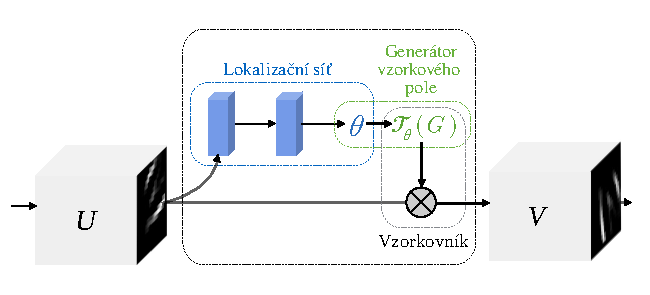
\includegraphics[width=0.8\textwidth,keepaspectratio]{Figures/stn/stn_module.pdf}
\caption[Zjednodušený pohled na STN modul]
{Zjednodušený pohled na STN modul, kde $U$ je vstupní obraz a $V$ je výstupní obraz. Lokalizační síť provádí regresi transformačních parametrů $\theta$, která je pak využita pro generaci vzorkového pole. Příkladná vizualizace vzorkového pole, a jeho použití ve vzorkovníku, je znázorněna na obrázku \ref{fig:stn_grid}. Převzato z \cite{stn} a upraveno. }
\label{fig:stn_overview}
\end{figure}

\subsection{Lokalizační síť}

První částí je \textbf{lokalizační síť} (ang. localization net). Právě tato část modulu je jako jediná trénovatelná. Vstupem do lokalizační sítě může být jakýkoli n-kanálový obraz či mapa příznaků. Výstup lokalizační sítě jsou parametry $\theta$ společné pro všechny kanály vstupního snímku. Architektura sítě není striktně dána, může být postavena jak na CNN nebo FCN za předpokladu, že finální část sítě bude uzpůsobena pro regresi parametrů afinní transformace $\theta$ reprezentovanou v matici ${\displaystyle \mathrm {A} }_\theta$.

Matice ${\displaystyle \mathrm {A} }_\theta$ může nabírat několika forem. Prvním klasickým přístupem může být následující matice $2\times3$:
\begin{equation}
    {\displaystyle \mathrm {A} }_\theta = 
    \begin{bmatrix}
        \theta_{11} & \theta_{12} & \theta_{13} \\
        \theta_{21} & \theta_{22} & \theta_{23}
    \end{bmatrix}
    \label{eq:stn_6_theta}
\end{equation}
pro translaci, rotaci, škálování a zkosení podél os. Matice ${\displaystyle \mathrm {A} }_\theta$ avšak může nabírat i více podob, jako např. 12-člennou matici $4\times3$ pro 3D afinní transformace nebo následující poupravenou afinní 2D matici pro prostorovou pozornost, umožňující translaci, izotropní škálování a ořezávání:

\begin{equation}
    {\displaystyle \mathrm {A} }_\theta = 
    \begin{bmatrix}
        s & 0 & t_x \\
        0 & s & t_y
    \end{bmatrix}.
    \label{eq:stn_3_theta}
\end{equation}

Ořezávání je dosaženo s pomocí levé $2\times2$ strany matice ${\displaystyle \mathrm {A} }_\theta$ zapsanou jako ${\displaystyle \mathrm {A'} }_\theta$. Pokud platí, že $determinant({\displaystyle \mathrm {A'} }_\theta) < 1.0$, pak je výsledná plocha transformace menší než plocha originálního vstupu a vzorkové pole se soustředí pouze na jistou část snímku, což vede k lokálnější prostorové pozornosti.

\subsection{Generátor vzorkového pole}

Výstup lokalizační sítě, matice ${\displaystyle \mathrm {A} }_\theta$, pak následuje do další části modulu STN - \textbf{generátoru vzorkového pole} (v originální ang. podobě grid generator). Generátor vzorkového pole generuje 2-složkové pole, které aplikuje parametry afinní transformace ${\displaystyle \mathrm {A} }_\theta$. K tomu se využívá způsob inverzního mapování.

\begin{figure}[h]
\centering
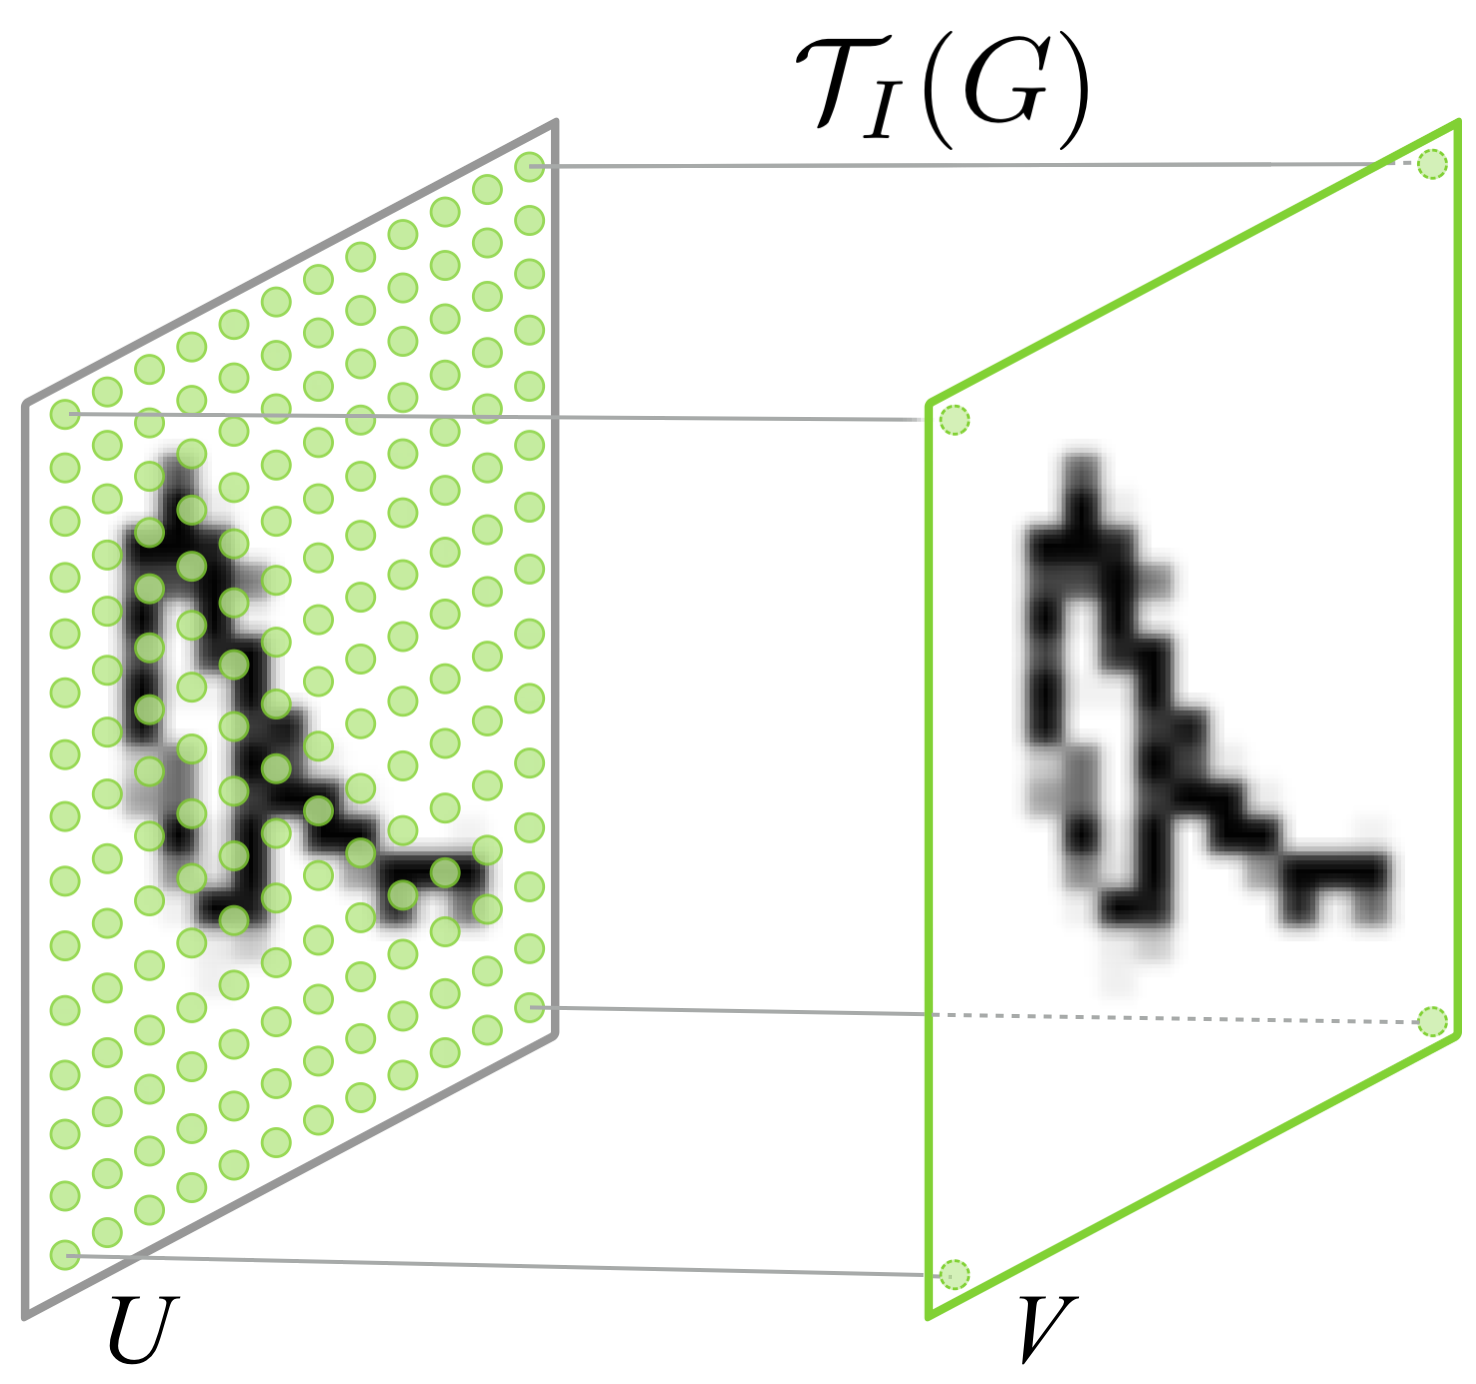
\includegraphics[width=0.3\textwidth,keepaspectratio]{Figures/stn/stn_a.png}
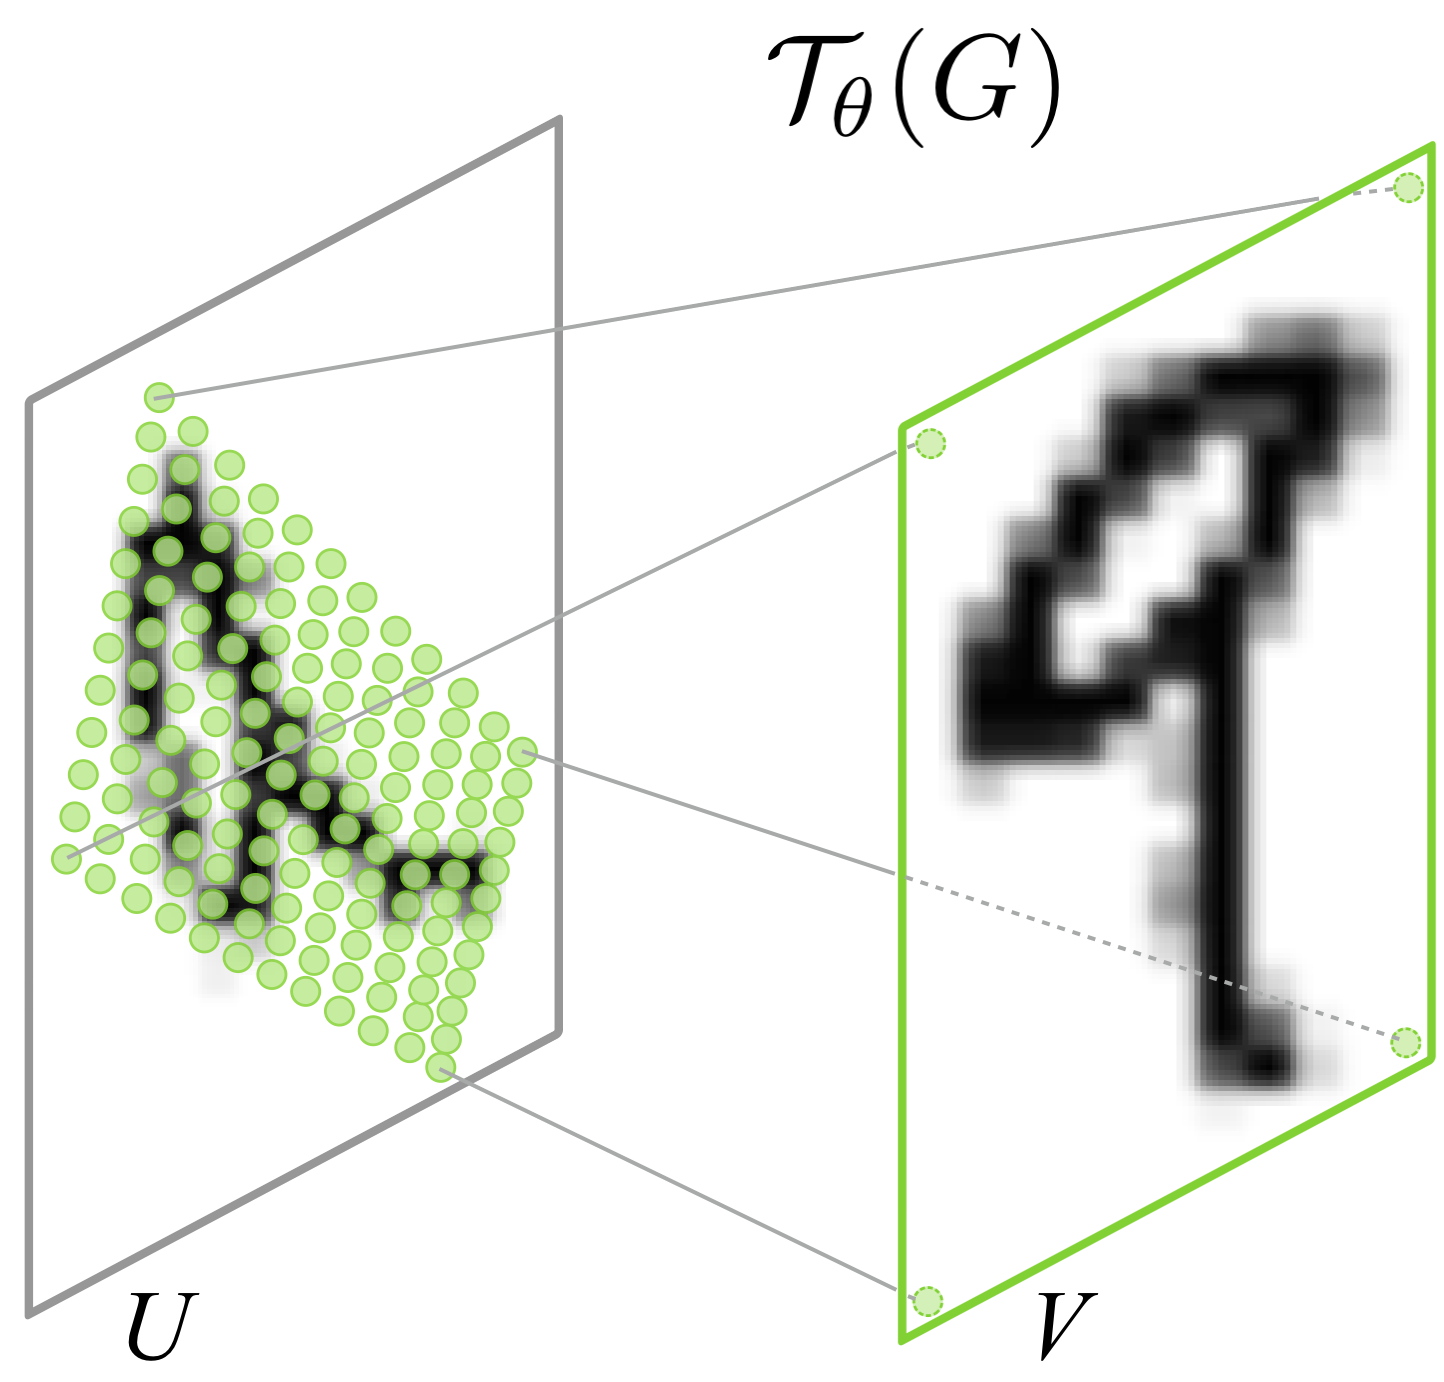
\includegraphics[width=0.3\textwidth,keepaspectratio]{Figures/stn/stn_b.png}
\caption[Vizualizace generování vzorkového pole v modulu STN]
{Vizualizace generování vzorkového pole v modulu STN a jeho aplikace na transformování vstupního snímku ve vzorkovníku, kde $T_{\theta}(G)$ je 2D skalární pole s transformovanými souřadnicemi pravidelné mřížky (ang. regular grid) $G$ zdrojového pole. $T_{I}(G)$ je jednotková transformace. Převzato z \cite{stn}. }
\label{fig:stn_grid}
\end{figure}

Inverzní mapování je často použito oproti přímému mapování, které nefunguje dobře díky přesahům a mezerám, které zanechá při mapování ve výsledném snímku. Inverzní mapování bývá standardním postupem v praxi při podobných úlohách počítačového vidění \cite{stn_medium_1}. Inverzní mapování v kontextu STN ve 2D prostoru může být (identicky jako v originální literatuře \cite{stn}) definováno takto:

\begin{equation}
\begin{pmatrix}
x_i^s \\
y_i^s
\end{pmatrix}
= T_{\theta}(G_i) = {\displaystyle \mathrm {A} }_\theta
\begin{pmatrix}
x_i^t \\
y_i^t \\
1
\end{pmatrix}
= 
\begin{bmatrix}
\theta_{11} & \theta_{12} & \theta_{13} \\
\theta_{21} & \theta_{22} & \theta_{23}
\end{bmatrix}
\begin{pmatrix}
x_i^t \\
y_i^t \\
1
\end{pmatrix},
\label{eq:stn_inverse}
\end{equation}
kde $(x_i^s, y_i^s)$ je daná pozice na původním obrazu, kterou počítáme pomocí funkce inverzního mapování na základě transformovaného vzorkového pole $T_{\theta}(G)$. To lze vyjádřit jako násobení matice ${\displaystyle \mathrm {A} }_\theta$ a cílové pozice v homogenní formě $(x_i^t, y_i^t, 1)$. Výsledkem použití inverzního mapování (ve funkci \ref{eq:stn_inverse}) je vzorkové pole reprezentované také jako 2D 2-složkové pole či dvě 2D skalární pole pro osy $(x, y)$.

\subsection{Vzorkovník}

Pro provedení prostorové transformace na originálním snímku modulu STN zde máme poslední část známou jako \textbf{vzorkovník} (v originální ang. podobě sampler). Vzorkovník společně se vstupním obrazem (nebo mapou příznaků) a vzorkovým polem generuje finální snímek modulu STN s aplikovanými prostorovými změnami. Vzorkovník využije vzorkové pole a s pomocí bilineární interpolace převede hodnoty pixelů z originálního snímku na transformovaný snímek finální, podobně jak je znázorněno na obrázku \ref{fig:stn_grid}. Je dobré podotknout, že velikost vzorkového pole přímo ovlivňuje velikost výstupního snímku. Pokud má snímek více kanálů, je transformace aplikována identicky na všechny kanály vstupního snímku \cite{stn_medium_3}.

Funkce vzorkovníku může být zjednodušeně pro mapování hodnot na základě nejbližší lokace (bez použití interpolace) znázorněna takto:
\begin{equation}
    V_i^c = \sum_{n=1}^{H} \sum_{m=1}^{W} U_{nm}^c \delta(\lfloor x_s^i + 0.5 \rfloor - m) \delta(\lfloor y_s^i + 0.5 \rfloor - n)\,,
\label{eq:stn_sampler_int}
\end{equation}
kde se zdrojové pozice $(x_i^s, y_i^s)$ mapují na výsledné pozice $(x_i^t, y_i^t)$ pro $V_i^c$, $U_{nm}^c$ je hodnota pixelu ve vstupním obrazu na dané pozici $(n, m)$ v kanálu $c$, $\delta$ je Kroneckerovo delta a pomocí posunu o hodnotě 0,5 se pozice zaokrouhlí na nejbližší celé číslo. Pro verzi s použitím bilineární interpolace se převod na základě předchozí funkce \ref{eq:stn_sampler_int} dá formulovat následovně:
\begin{equation}
    V_i^c = \sum_{n=1}^{H} \sum_{m=1}^{W} U_{nm}^c \max(0, 1 - |x_s^i - m|) \max(0, 1 - |y_s^i - n|)\,.
\label{eq:stn_sampler_bi}
\end{equation}

\subsection{Zpětná propagace STN}

Funkce \ref{eq:stn_sampler_bi} pro vzorkovaní pozic ze zdroje na cíl je diferenciovatelná pro všechny hodnoty na výsledné mapě $V$. Je možno použít i jiné kernelové funkce\footnote{Označení pro funkci vzorkovníku \cite{stn}.} pro převod těchto pozic a hodnot za předpokladu zachování diferenciovatelnosti pro účely zpětné propagace. Pro funkce generující výslednou mapu $V_i^c$ je možno odvodit následné parciální derivace vzhledem vůči zdrojovému obrazu $\frac{\delta V_i^c}{\delta U_{nm}^c}$ a také i vůči zdrojovým pozicím $\frac{\delta V_i^c}{\delta x_i^s}$, resp. $\frac{\delta V_i^c}{\delta y_i^s}$. Toto umožňuje propagaci gradientů jak do zdrojového obrazu $U_{nm}^c$, tak do pozic vzorkového pole $(x_i^s, y_i^s)$. Zpětná propagace díky tomu dosahuje i do lokalizační sítě, jelikož parciální derivace $\frac{\delta x_i^s}{\delta \theta}$ a $\frac{\delta y_i^s}{\delta \theta}$ jsou schopny být odvozeny a zderivovány z funkce \ref{eq:stn_inverse}. Díky této vlastnosti může být modul STN vložen do existujících sítí a být jednoduše natrénován v rámci sítě jako celku (tzv. end-to-end\footnote{Proces trénování celého modelu jako jednoho celku od vstupu po výstup.}) \cite{stn}. 
\endinput